
\chapter{Bidirectional Radiance Caching}
\label{chap:bidirectional_caching}

\section{A General Theoretical Framework for Radiance Caching}
Before proposing new radiance caching techniques, I first want to take a step back and analyze radiance caching in general.

Radiance caching generally can be broken down into four steps:

\begin{enumerate}
    \item \textbf{Training}
    \begin{enumerate}
        \item \textbf{Query Prediction} First, we want to predict potential queries $\hat{q} = (\vec{x}, \vec{\omega}_o)$ according to a distribution $\hat{Q}(\hat{q})$.
        \item \textbf{Radiance Estimation} Given a predicted query $\hat{q}$, we want to estimate the outgoing radiance $L_o(\hat{q})$ at that query.
        For this, we can use any possible combination of radiance estimation techniques, such as path tracing, light tracing, photon mapping or bidirectional path tracing (BDPT).
    \end{enumerate}
    \item \textbf{Inference}
    \begin{enumerate}
        \item \textbf{Query Sampling} We sample queries $q = (\vec{x}, \vec{\omega}_o)$ according to a distribution $Q(q)$.
        \item \textbf{Interpolation} Given a query $q$, we want to approximate the outgoing radiance $\hat{L}_o(q)$ by interpolating the radiance estimates of spatio-temporally nearby query predictions $\hat{q}$.
        We can use any combination of storing and interpolation technique for this, such as nearest neighbor, linear interpolation or, in our case, the NRC.
        Note however, that this step generally introduces \textbf{bias}.
    \end{enumerate}
\end{enumerate}

\paragraph{Note:}
\label{par:cache_efficiency}
Using this framework we can observe that the \textbf{cache efficiency} is optimal if the query prediction distribution $\hat{Q}(\hat{q})$ is equal to the query sampling distribution $Q(q)$.
Conversely, if we sample a query $q^*$ that can not be predicted by the query predictor (i.e. $\hat{Q}(q^*)=0$), we introduce fundamental bias into the radiance cache $\hat{L}_o(q^*)$, because the radiance cache will not contain an accurate radiance estimate for that query.
This happens, whenever the support of the query sampling distribution $Q$ is not contained in the support of the query prediction distribution $\hat{Q}$, i.e. $\supp(Q) \not\subseteq \supp(\hat{Q})$.

\paragraph{Discussion:} It may be possible, to derive a better radiance cache by storing the incoming radiance and BSDFs in a data structure and connecting to them stochastically through ReSTIR DI \bcite{bitterli2020} similar to Virtual Point Lights in Instant Radiosity techniques \bcite{keller1997}.
% Or VCM

The general idea of decoupling radiance estimation and visualization was already explored by others, notably \textcite{walter1999} and \textcite{tole2002}.

\section{The Path Space Integral Formulation}
\label{sec:path_space_integral}
To be able to robustly derive the following radiance estimators, I will use an alternative but equivalent formulation of the rendering equation as an integral over the path space, which was first introduced by \textcite{veach1997}.
\begin{figure}[ht]
    \centering
    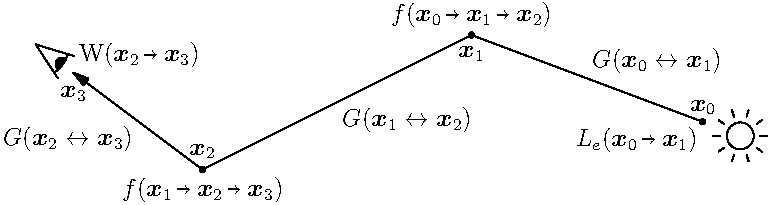
\includegraphics{asy/path_integral.pdf}
\caption{Radiance transfer along a path of length $n=3$ according to the path space integral formulation.}
\label{fig:path_space_integral}
\end{figure}

A path $\bar{x}$ of length $n$ is defined as a sequence of vertices $\vec{x}_0 \vec{x}_1 \dots \vec{x}_n$.
Let the space of all paths of length $n$ be $X_n$ and the space of all paths $X = \bigcup_{n=1}^{\infty} X_n$.
Then, the path space integral formulation of the rendering equation is given by:
\begin{equation}
\label{eq:path_space_integral}
\begin{aligned}
    I
    = \sum_{n=0}^{\infty} \int_{X_n} L_e(\pdir{0}{1}) \G{0}{1} &\prod_{i=1}^{n - 1} \f{i-1}{i}{i+1} \G{i}{i+1}\\
    &\cdot W(\pdir{n-1}{n}) \diff A(\vec{x}_0) \dots \diff A(\vec{x}_n)
\end{aligned}
\end{equation}
To collect incoming radiance at a sensor point $\vec{x}_n$, the path space integral formulation contains a sensor weighting term $W(\pdir{n-1}{n})$, which in the case of an infinitesimal pin-hole camera is simply a Dirac-Delta-function over the eye position and a box function over the viewing directions covered by the pixel.
The arrow notation $\vec{x} \pto \vec{y}$ denotes a ray starting at $\vec{x}$ traveling towards $\vec{y}$, i.e. $L_o(\vec{x} \pto \vec{y}) \defeq L_o(\vec{x}, \vec{y} - \vec{x})$.
The triples represent surface interactions, $f(\vec{x} \pto \vec{y} \pto \vec{z}) \defeq f(\vec{y} - \vec{x}, \vec{y}, \vec{z} - \vec{y})$. 
Double arrow notation is used for path segments, $G(\vec{x} \leftrightarrow \vec{y})$ models the radiance transfer between the vertices $\vec{x}$ and $\vec{y}$:
\begin{equation}
\label{eq:transfer}
G(\vec{x} \leftrightarrow \vec{y}) \defeq V(\vec{x} \leftrightarrow \vec{y}) \frac{\cos \theta_{\vec{x} \veryshortarrow \vec{y}} \cos \theta_{\vec{y} \veryshortarrow \vec{x}}}{\|\vec{y} - \vec{x}\|^2},
\end{equation}
where $V(\vec{x} \leftrightarrow \vec{y}) \in \{0,1\}$ defines visibility and $\theta$ denotes the respective angles of incidence.
The integral is measured over the surface of the scene $A(\vec{x})$.

\begin{figure}[ht]
    \centering
    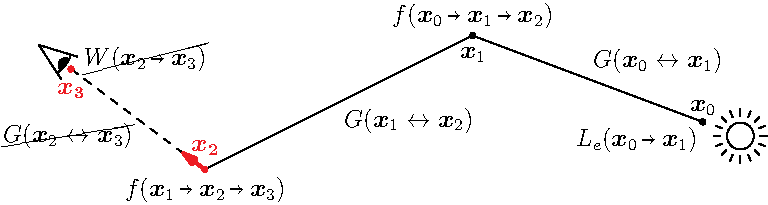
\includegraphics{asy/path_integral_radiance.pdf}
\caption{To estimate the outgoing radiance $L_o(\pdir{2}{3})$ with the path space integral formulation, we fix the last two vertices defining the position and direction, here $\vec{x}_2$ and $\vec{x}_3$ highlighted in red. Furthermore, we drop the sensor weighting term $W$ and the last geometry term $\G{2}{3}$, because they are not part of the path anymore.}
\label{fig:path_space_integral_radiance}
\end{figure}
In the following derivations, I will also use a slightly adapted formulation of the path space integral, that estimates \emph{radiance} instead of \emph{intensity} (see \autoref{fig:path_space_integral_radiance}).
Therefore, we only have to drop the sensor weighting term $W$ and the last geometry term $\G{n-1}{n}$ and fix the last two vertices, which define the position and direction of outgoing radiance, by excluding them from the integration domain:
\begin{equation}
\label{eq:path_space_integral_radiance}
\begin{aligned}
    % L_o(x, \wo) = \sum_{n=0}^{\infty} \int_{X_n} L_e(\pdir{0}{1}) \G{0}{1} \prod_{i=1}^{n - 1} \f{i-1}{i}{i+1} \G{i}{i+1}\\
    % \f{n-1}{n}{} \G{n}{} f(\vec{x}_n \pto \vec{x}, \wo) \ \diff A(\vec{x}_0) \dots \diff A(\vec{x}_n)
    L_o(\pdir{n-1}{n})
    %= L_i(\pdir{n-1}{n})
    = &\sum_{n=0}^{\infty} \int_{X_{n-2}} L_e(\pdir{0}{1}) \\
    &\cdot \prod_{i=1}^{n - 1} \G{i-1}{i} \f{i-1}{i}{i+1} 
    \diff A(\vec{x}_0) \dots \diff A(\vec{x}_{n-2})
\end{aligned}
\end{equation}

The main advantage of these formulations is the independence of the individual vertices.
This for example allows for straightforward bidirectional sampling.
An essential tool for the derivation of path samplers is the conversion between area and solid angle measure, given by:
\begin{equation}
\label{eq:area_solid_angle}
\diff A(\vec{y}) = \frac{\cos \theta_{\vec{y}\veryshortarrow\vec{x}}}{\|\vec{y} - \vec{x}\|^2} \diff \omega(\vec{x}\pto\vec{y}),
\end{equation}
or directly applied to sampling probabilities:
\begin{equation}
\label{eq:area_solid_angle_p}
p(\vec{y}) = \frac{\cos \theta_{\vec{y}\veryshortarrow\vec{x}}}{\|\vec{y} - \vec{x}\|^2} p(\vec{x}\pto\vec{y}).
\end{equation}

\section{Inference}
\label{sec:inference}
Using this framework a simple inference scheme naturally emerges from the Path Space Integral Formulation (\autoref{eq:path_space_integral}).
The path length $n$ is limited by a path termination strategy (\autoref{sec:path-termination}), so we only need to calculate the finite sum up to the termination length $l$ because we terminate with a valid radiance estimate which incorporates the sum over longer paths.
We replace the integral over the path space $X_n$ by a primary Monte-Carlo Estimator.
For readability, I will do an exemplary derivation for a path of length $n=2$ without intermediate emission:
\begin{subequations}
\begin{align}
    % Length n=2
    I
    &= \int_{X_n} \widehat{L}_o(\pdir{0}{1}) \G{0}{1} \f{0}{1}{2} \G{1}{2} \cancel{W(\pdir{1}{2})} \diff A(\vec{x}_0) \!\cdots\! \cancel{\diff A(\vec{x}_2)}\notag\\
    &= \int_{X_{n-1}} \widehat{L}_o(\pdir{0}{1}) \G{0}{1} \f{0}{1}{2} \G{1}{2} \diff A(\vec{x}_0) \diff A(\vec{x}_1) \label{eq:cancelw}\\
    &\eqhat \frac{\widehat{L}_o(\pdir{0}{1}) \G{0}{1}}{p(x_0)}  \frac{\f{0}{1}{2} \G{1}{2}}{p(x_1)} \label{eq:pmc}\\
    &= \frac{\widehat{L}_o(\pdir{0}{1}) \cos\theta_{1\veryshortarrow0}}{p(\pdir{1}{0}\mid\pdir{2}{1})}  \frac{\f{0}{1}{2} \cos\theta_{2\veryshortarrow1}}{p(\pdir{2}{1})} \label{eq:area2solid}
    % Length n=3
    % I
    % &= \int_{X_n} \widehat{L}_o(\pdir{0}{1}) \G{0}{1} \f{0}{1}{2} \G{1}{2} \f{1}{2}{3} \G{2}{3} \delta(\pdir{2}{3}) \diff A(\vec{x}_0) \dots \diff A(\vec{x}_3)\\
    % &= \int_{X_{n-1}} \widehat{L}_o(\pdir{0}{1}) \G{0}{1} \f{0}{1}{2} \G{1}{2} \f{1}{2}{3} \G{2}{3} \diff A(\vec{x}_0) \dots \diff A(\vec{x}_2)\\
    % &\approx \frac{\widehat{L}_o(\pdir{0}{1}) \G{0}{1}}{p(x_0)}  \frac{\f{0}{1}{2} \G{1}{2}}{p(x_1)} \frac{\f{1}{2}{3} \G{2}{3}}{p(x_2)}\\
    % &= \frac{\widehat{L}_o(\pdir{0}{1}) \cos\theta_{0\veryshortarrow1}}{p(\pdir{1}{0}\mid\pdir{2}{1})}  \frac{\f{0}{1}{2} \cos\theta_{1\veryshortarrow2}}{p(\pdir{2}{1}\mid\pdir{3}{2})} \frac{\f{1}{2}{3} \cos\theta_{2\veryshortarrow3}}{p(\pdir{3}{2})}\\
\end{align} % TODO: generic
\end{subequations}
In the first step, the sensor weighting term $W$ cancels with the integration over the eye vertex (\ref{eq:cancelw}).
We then replace the integral by a primary Monte Carlo estimator (\ref{eq:pmc}).
Finally, we convert from area measure to solid angle measure using (\autoref{eq:area_solid_angle_p}) which cancels with $G$ leaving only the cosine terms at the sampled vertices (\ref{eq:area2solid}).
The visibility term implicitly vanishes in the ray tracing step.
\begin{figure}[ht]
    \centering
    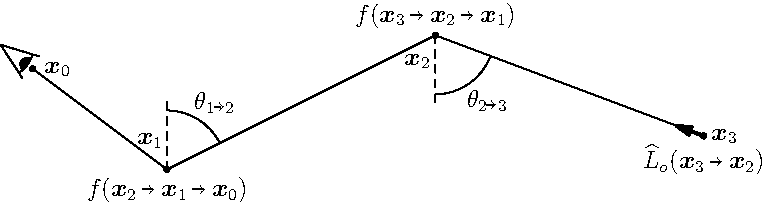
\includegraphics{asy/inference.pdf}
\caption{Visualization of the inference process.}
\label{fig:inference}
\end{figure}

Applying these observations to all path lengths up to termination, we get:
\begin{equation}
\label{eq:inference}
    I
    \hateq \sum_{i=1}^{n-1} T_i L_e(\pdir{i}{i-1}) + T_n \widehat{L}_o(\pdir{n}{n-1}), \quad
    T_n
    = \prod_{i=1}^{n} \frac{f(\ptrip{i-1}{i}{i+1}) \cos \theta_{i \veryshortarrow i+1}}{p(\pdir{i}{i+1} \mid \pdir{i-1}{i})}
\end{equation}
where $T_n$ is the accumulated throughput along the first $n$ segments of the path and $\widehat{L}_o(\pdir{n}{n-1})$ is the interpolated radiance estimate at the termination vertex.
To simplify notation, the path now starts at the eye vertex $\vec{x}_0$.
Note, that Russian Roulette Termination (\autoref{eq:rr}) is not to be applied here, as we terminate the path with a valid radiance estimate.

\section{Path Tracing}
\label{sec:re_eye}
\begin{figure}[ht]
    \centering
    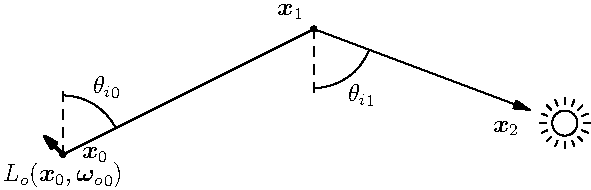
\includegraphics{asy/eye_tracing.pdf}
\caption{The simplest way to estimate the outgoing radiance $L_o(\x_0, \wo_0)$ is eye tracing, which shoots a path from the surface into the scene and collects emissions at each intersection.}
\label{fig:eye_tracing}
\end{figure}
We can apply the observations made in \autoref{sec:inference} to the path space formulation for radiance (\autoref{eq:path_space_integral_radiance}) to derive a path tracing based radiance estimator:
\begin{equation}
    L_o(\vec{x}_0, \wo_0)
    \hateq \sum_{k=1}^{\infty} T_k L_e(\vec{x}_k, \wo_k), \quad
    T_n
    = \prod_{k=0}^{n-1} \frac{f(\wi_k, \x_k, \wo_k) \cos {\theta_i}_k}{p(\wi_k \mid \wo_k)}
\end{equation}

\begin{figure}[ht]
    \centering
    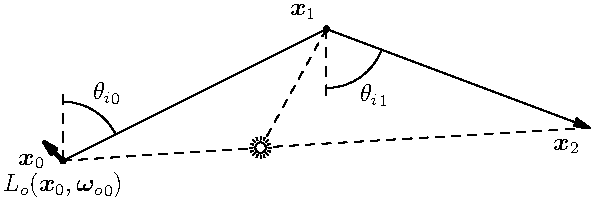
\includegraphics{asy/nee.pdf}
\caption{Direct light sampling also known as Next Event Estimation (NEE) performs significantly better than BSDF sampling on small direct lighting.}
\label{fig:nee}
\end{figure}
This estimator alone however is ineffective at finding small light sources, so we combine it with Next Event Estimation through Multiple Importance Sampling (\autoref{sec:mis}), as we already did in the reference pathtracer:
\begin{equation}
\begin{aligned}
    L_o(\vec{x}_0, \wo_0)
    \hateq \sum_{k=1}^{\infty} T_k \left( w_\text{BSDF} L_e(\x_k, \wo_k) + w_\text{L} \frac{f(\pdir{L}{k}, \wo_k) \G{k}{L} L_e(\pdir{L}{k})}{p(\x_L)} \right)
\end{aligned}
\end{equation}
By combining the two techniques by weighting them with their respective MIS-weights $w_\text{BSDF}(\wo)$ and $w_\text{L}(\x_L)$ (\autoref{eq:balance_heuristic} and \autoref{eq:power_heuristic}), we get the best of both worlds.
This combined with ReSTIR DI \bcite{bitterli2020} and a LightBVH \bcite{moreau2019} for efficient many light sampling is the radiance estimator used by \textcite{muller2021}.
However, I simply sample the light source from a precomputed CDF-table by inversion sampling, because my test scenes only contain a few light sources.
To limit the path length, I use Russian Roulette Termination (\autoref{eq:rr}) again, and in praxis the path length also has to be limited to a maximum length, which introduces potential bias.

\section{Bidirectional Training}
\label{sec:re_bidir}
A major weakness of the aforementioned radiance estimator (\autoref{sec:re_eye}) is indirect lighting where the light paths undergo glossy reflections/refractions before getting diffused.
This effect is known as a caustic.
In the extreme case of an infinitesimal light source being ideally reflected/refracted and then diffused, path tracing and NEE even fail completely to capture this effect, because the probability to sample such a path by BSDF sampling is zero.
However, we can do the exact opposite of NEE by tracing light paths and connecting them to query points sampled from the eye.
This technique elegantly resolves even long glossy light paths.

\begin{figure}[ht]
    \centering
    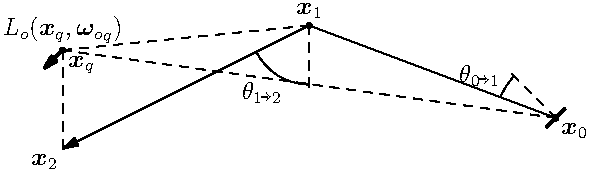
\includegraphics{asy/bidir.pdf}
\caption{Flux is distributed along a BSDF-sampled path from a random point on a light source ($\x_0$). At the query point $\x_q$ radiance is collected by deterministically connecting to every vertex of the light path.}
\label{fig:bidir}
\end{figure}
Specifically, I propose the following alternative radiance estimator based on this idea:
First, sample a query point $q = (\vec{x}_q, \wo_q)$ from the query sampling distribution $Q(q)$.
Then, trace a light path carrying flux from a randomly selected light source via BSDF sampling and connect each vertex $\vec{x}_k$ to the query point $\vec{x}_q$.

Starting again with the Primary Monte Carlo Estimator for the Path Space Integral for Radiance (\autoref{eq:path_space_integral_radiance}) and applying the same observations as in \autoref{sec:inference}, we get:
\begin{equation}
\label{eq:bidir}
\begin{aligned}
    L_o(\vec{x}_q, \wo_q)
    &\hateq \frac{L_e(\pdir{0}{q})}{p(\x_0)} \G{0}{q} f(\pdir{0}{q}, \wo_q) \\
    &+ \sum_{k=1}^{\infty} \Phi_k \cdot \f{k-1}{k}{q} \G{k}{q} f(\pdir{k}{q}, \wo_q), \\
    \Phi_n &= \frac{L_e(\pdir{0}{q}) \cos \theta_{0 \veryshortarrow 1}}{p(\x_0) p(\pdir{0}{1})} \prod_{i=2}^{n} \frac{f(\ptrip{i-1}{i}{i+1}) \cos \theta_{i \veryshortarrow i+1}}{p(\pdir{i}{i+1} \mid \pdir{i-1}{i})},
\end{aligned}
\end{equation}
where $\Phi_n$ is the light flux transported along the path.
The sum over the path length is split into two parts because the first vertex $\vec{x}_0$ is sampled directly on the light source and requires special handling.

In practice, I only sample queries by shooting primary camera rays, because this is already a good approximation of the query sampling distribution $Q(q)$.

\section{Light Tracing}
\label{sec:light_tracing}
However, despite already sampling light paths, the estimator from \autoref{sec:re_bidir} only finds indirect illumination by caustics efficiently, since given a specific query, the probability to connect to a glossy light path directly is still low.
So, instead of predicting queries solely from the eye, we can also collect radiance at future vertices of the light path.
At a light vertex, we are guaranteed to get strong contribution at least from the previous vertex, because we sampled it directly through BSDF sampling.
It would also be possible to sample independent queries from the light vertices instead of reusing the next light vertex and this may in fact be an interesting algorithm to explore, though this is outside the scope of this thesis.

\paragraph{Balancing} Although this estimator may look promising at first, it is important to note that it exhibits the problem already discussed in my motivation of bidirectional radiance caching (\autoref{par:cache_efficiency}):
By sampling queries solely from the light, queries that are shadowed will never be predicted, which introduces bias into the cache.
This can be clearly visible depending on the scene and will be further discussed in the results chapter (\autoref{chap:results}).

To counteract this drawback, we can make a simple observation:
If a query is not reachable from a light source, it does not receive energy, thus the radiance at such queries can be safely assumed to be zero.
Because the Neural Radiance Cache performs averaging in local neighborhoods, we can carefully introduce samples with radiance zero according to the query sampling distribution $Q(q)$.
By weighting the valid samples with the inverse of the ratio of zero samples, we can ensure that the mean over a local neighborhood is still correct:
\begin{equation}
\expectationvar{q}{{\widehat{L}_o}(\vec{x}_q, \wo_q)} = p_0 \cdot 0 + \frac{1}{n} \sum_{q \in Q} \frac{1}{p_0} L_o(\vec{x}_q, \wo_q) = \widehat{L}_o(\vec{x}_q, \wo_q)
\end{equation}

Essentially this algorithm models a sort of output decay on the NRC, dragging its prediction towards zero.
This can work, but it degrades the quality of the cache, since it introduces additional noise with the zero radiance samples.
Furthermore, it is a waste of bandwidth to spend resources on learning zero radiance, as it does not provide any information gain.

\section{Path Spaced Denoised Sparse Photon Mapping}
\label{sec:psdpm}
The final radiance estimator I propose is an adaptation of Photon Mapping by \textcite{jensen1996}.
We again shoot flux into the scene by light tracing.
However, instead of collecting the flux by connecting to an infinitesimal query point, we collect the incoming flux over all sampled light paths in a \emph{query region} by kernel density estimation.
\begin{subequations}
\begin{align}
    L_o(\x, \wo)
    &= \int_{\Omega_i} f(\wi, \x, \wo) L_i(\wi, \x) \cos{\theta_i} \diff\wi \label{eq:pm:lo}\\
    &= \int_{\Omega_i} f(\wi, \x, \wo) \frac{\diff^2 \Phi_i(\wi, \x)}{\diff A \; \cancel{\cos{\theta_i} \diff\wi}} \cancel{\cos{\theta_i} \diff\wi} \label{eq:pm:defrad}\\
    &\hateq \frac{1}{n} \sum_{i=1}^n f(\hat{\vec{\omega}}_i, \x, \wo) \frac{\Delta \Phi_i(\hat{\vec\omega}_i, \x)}{\Delta A} \label{eq:pm:est}\\
    &\approx \frac{1}{n \pi r^2} \sum_{i=1}^n f(\hat{\vec{\omega}}_i, \x, \wo) \Delta \Phi_i(\hat{\vec\omega}_i, \x) \label{eq:pm:sphere}
\end{align}
\end{subequations}
We start with the rendering equation (\ref{eq:pm:lo}) and replace the incoming radiance $L_i$ by its definition as incoming flux per area and solid angle (\ref{eq:pm:defrad}).
We then replace the integral by a Monte Carlo estimator over $n$ sampled flux packages \emph{(photons)} (\ref{eq:pm:est}).
Finally, we use a box function inside a sphere of radius $r$ as our kernel.
Assuming the surface is locally flat, this allows us to approximate the surface area $\Delta A$ over which we are integrating by a disk of area $A=\pi r^2$ (\ref{eq:pm:sphere}).

\paragraph{Hardware Acceleration}

%\section{Hardware Accelerated Vertex Connection and Merging}